\documentclass[11pt]{article}
\newif\ifko\kofalse
\newcommand{\shorttitle}{Foreground-protecting resource orchestration for Windows}
% Shared preamble for the Korean and English RamFlow papers.
% Each main file defines \ifko (true for Korean) before \input-ing this file.
\usepackage[a4paper,top=24mm,bottom=26mm,left=25mm,right=25mm,headsep=8mm,footskip=11mm]{geometry}
\usepackage{amsmath,amssymb}
\usepackage{mathpazo}
\usepackage[no-math]{fontspec}
\ifko
  % Korean: Noto CJK KR carries both Hangul and Latin glyphs, so one family
  % keeps the colour of the page even. Lines break at inter-word spaces.
  \setmainfont{Noto Serif CJK KR}[Scale=0.94,BoldFont={* SemiBold}]
  \setsansfont{Noto Sans CJK KR}[Scale=0.92,BoldFont={* Bold}]
  \setmonofont{DejaVu Sans Mono}[Scale=0.80]
  \linespread{1.30}
  \XeTeXlinebreaklocale "ko"
  \XeTeXlinebreakskip=0pt plus 0.6pt
  \AtBeginDocument{\renewcommand{\emph}[1]{\textsf{#1}}}
  % inside diagrams and tables, break only at spaces and never letter-space
  \AtBeginDocument{\tikzset{every picture/.append style={execute at begin picture={\XeTeXlinebreaklocale ""\XeTeXlinebreakskip=0pt\relax},execute at end picture={\XeTeXlinebreaklocale "ko"}}}}
  \renewcommand{\figurename}{그림}
  \renewcommand{\tablename}{표}
  \renewcommand{\contentsname}{차례}
  \renewcommand{\appendixname}{부록}
  \renewcommand{\abstractname}{초록}
  \AtBeginDocument{\floatname{algorithm}{알고리즘}}
  \AtBeginDocument{\renewcommand{\figurename}{그림}\renewcommand{\tablename}{표}}
\else
  \setmainfont{TeX Gyre Pagella}
  \setsansfont{Noto Sans CJK KR}[Scale=0.92]
  \setmonofont{DejaVu Sans Mono}[Scale=0.80]
  \linespread{1.12}
\fi
\usepackage{microtype}
\setlength{\emergencystretch}{1.5em}
\usepackage{xcolor}
\definecolor{accent}{HTML}{2A78D6}
\definecolor{offc}{HTML}{EB6834}
\definecolor{ink2}{HTML}{52514E}
\definecolor{rule}{HTML}{D9D8D3}
\definecolor{panel}{HTML}{F4F3F0}
\usepackage{graphicx}
\usepackage{booktabs,tabularx,multirow,array}
\usepackage{caption}
\captionsetup{font=small,labelfont={bf,sf},labelsep=period,skip=5pt}
\usepackage{enumitem}
\setlist{itemsep=1pt,topsep=3pt,leftmargin=1.6em}
\usepackage{tikz}
\usetikzlibrary{arrows.meta,positioning,fit,calc,backgrounds,shapes.geometric}
\usepackage{algorithm}
\usepackage[noend]{algpseudocode}
\usepackage{titlesec}
\titleformat{\section}{\large\sffamily\bfseries}{\color{accent}\thesection}{0.8em}{}
\titleformat{\subsection}{\normalsize\sffamily\bfseries}{\color{accent}\thesubsection}{0.7em}{}
\titleformat{\paragraph}[runin]{\normalsize\sffamily\bfseries}{}{}{}[.]
\titlespacing*{\section}{0pt}{14pt plus 3pt}{6pt}
\titlespacing*{\subsection}{0pt}{10pt plus 2pt}{4pt}
\titlespacing*{\paragraph}{0pt}{6pt plus 1pt}{0.6em}
\usepackage{fancyhdr}
\pagestyle{fancy}\fancyhf{}
\renewcommand{\headrulewidth}{0pt}
\fancyhead[L]{\footnotesize\sffamily\color{ink2}RamFlow}
\fancyhead[R]{\footnotesize\sffamily\color{ink2}\shorttitle}
\fancyfoot[C]{\footnotesize\sffamily\color{ink2}\thepage}
\fancypagestyle{plain}{\fancyhf{}\fancyfoot[C]{\footnotesize\sffamily\color{ink2}\thepage}}
\usepackage[hidelinks,unicode]{hyperref}
\hypersetup{colorlinks=true,linkcolor=accent,citecolor=accent,urlcolor=accent}
\usepackage{xurl}
\usepackage[numbers,sort&compress]{natbib}
\setlength{\bibsep}{2pt plus 1pt}
\renewcommand{\bibfont}{\small}
\tikzset{prose/.style={}}
\ifko\tikzset{prose/.style={execute at begin picture={\XeTeXlinebreaklocale "ko"\XeTeXlinebreakskip=0pt plus 0.6pt\relax}}}\fi
\newcommand{\KoEn}[2]{\ifko #1\else #2\fi}
\newcommand{\code}[1]{\texttt{#1}}
\newcommand{\pct}{\%}
% Generated by paper/analysis/analyze.py -- do not edit by hand.
\newcommand{\numCSOff}{88.15}
\newcommand{\numCSOn}{48.14}
\newcommand{\numCSRed}{45.4}
\newcommand{\numCSBlkMed}{41.0}
\newcommand{\numCSBlkMin}{39.2}
\newcommand{\numCSBlkMax}{57.3}
\newcommand{\numCSGmRed}{46.5}
\newcommand{\numCSGmLo}{34.9}
\newcommand{\numCSGmHi}{55.9}
\newcommand{\numCSOffFifty}{76.55}
\newcommand{\numCSOnFifty}{38.73}
\newcommand{\numCOOff}{88.56}
\newcommand{\numCOOn}{48.95}
\newcommand{\numCORed}{44.7}
\newcommand{\numCOBlkMed}{39.6}
\newcommand{\numCOBlkMin}{37.2}
\newcommand{\numCOBlkMax}{53.2}
\newcommand{\numCOGmRed}{43.3}
\newcommand{\numCOGmLo}{33.6}
\newcommand{\numCOGmHi}{51.5}
\newcommand{\numCOOffFifty}{76.44}
\newcommand{\numCOOnFifty}{39.35}
\newcommand{\numVCOff}{99.36}
\newcommand{\numVCOn}{50.52}
\newcommand{\numVCRed}{49.2}
\newcommand{\numVCBlkMed}{45.4}
\newcommand{\numVCBlkMin}{43.7}
\newcommand{\numVCBlkMax}{58.1}
\newcommand{\numVCGmRed}{50.5}
\newcommand{\numVCGmLo}{40.4}
\newcommand{\numVCGmHi}{58.9}
\newcommand{\numVCOffFifty}{65.14}
\newcommand{\numVCOnFifty}{38.80}
\newcommand{\numVSOff}{62.46}
\newcommand{\numVSOn}{31.60}
\newcommand{\numVSRed}{49.4}
\newcommand{\numVSBlkMed}{35.8}
\newcommand{\numVSBlkMin}{26.3}
\newcommand{\numVSBlkMax}{63.7}
\newcommand{\numVSGmRed}{43.4}
\newcommand{\numVSGmLo}{19.1}
\newcommand{\numVSGmHi}{60.4}
\newcommand{\numVSOffFifty}{34.97}
\newcommand{\numVSOnFifty}{23.50}
\newcommand{\numBgCOff}{267,405}
\newcommand{\numBgCOn}{107,056}
\newcommand{\numBgCRed}{60.0}
\newcommand{\numBgVOff}{220,064}
\newcommand{\numBgVOn}{87,371}
\newcommand{\numBgVRed}{60.3}
\newcommand{\numEfSOff}{72.70}
\newcommand{\numEfSOn}{44.40}
\newcommand{\numEfOOff}{83.00}
\newcommand{\numEfOOn}{46.90}
\newcommand{\numSessions}{10}
\newcommand{\numSessionsOk}{10}
\newcommand{\numPooledP}{0.0020}
\newcommand{\numTasks}{1,200}
\newcommand{\numConditions}{20}
\newcommand{\numMxOff}{232.85}
\newcommand{\numMxOn}{131.32}
\newcommand{\numMxRed}{43.6}
\newcommand{\numMxBlkMin}{39.7}
\newcommand{\numMxBlkMax}{43.8}
\newcommand{\numMxGmLo}{40.3}
\newcommand{\numMxGmHi}{44.6}
\newcommand{\numMxOffFifty}{223.60}
\newcommand{\numMxOnFifty}{129.01}
\newcommand{\numMxFiftyRed}{42.3}
\newcommand{\numMxBgRed}{59.6}
\newcommand{\numMxAvLo}{856.8}
\newcommand{\numMxAvHi}{1144.0}
\newcommand{\numCpOff}{230.78}
\newcommand{\numCpOn}{219.76}
\newcommand{\numCpRed}{4.8}
\newcommand{\numCpBlkMin}{0.9}
\newcommand{\numCpBlkMax}{6.0}
\newcommand{\numCpGmLo}{1.8}
\newcommand{\numCpGmHi}{6.6}
\newcommand{\numCpOffFifty}{227.62}
\newcommand{\numCpOnFifty}{128.99}
\newcommand{\numCpFiftyRed}{43.3}
\newcommand{\numCpBgRed}{38.4}
\newcommand{\numCpAvLo}{14425.9}
\newcommand{\numCpAvHi}{15157.5}
\newcommand{\numScAmb}{1,811.26}
\newcommand{\numScAbs}{1,896.05}
\newcommand{\numScDry}{1,853.10}
\newcommand{\numScLive}{1,877.65}
\newcommand{\numScDiff}{−18.40}
\newcommand{\numScDiffPct}{−0.97}
\newcommand{\numCiLevel}{93.8}
\newcommand{\numSignP}{0.0312}
\newcommand{\numWilP}{0.0625}

% A rounded "finding" box used for key takeaways
\newcommand{\finding}[1]{%
  \par\smallskip\noindent
  \begin{tikzpicture}[prose]
    \node[fill=panel,rounded corners=3pt,inner sep=7pt,text width=\dimexpr\linewidth-14pt\relax,align=left]{\small #1};
    \fill[accent,rounded corners=1pt] ($(current bounding box.north west)+(0,-1pt)$) rectangle ($(current bounding box.south west)+(2.2pt,1pt)$);
  \end{tikzpicture}\par\smallskip}

\graphicspath{{../figures/}}

\begin{document}
\thispagestyle{plain}

\begin{center}
{\sffamily\bfseries\LARGE RamFlow\par}
\vspace{4pt}
{\sffamily\large Protecting the Task in Use Instead of Emptying Memory:\\Conservative, Reversible Resource Orchestration on Windows\\and a Single-PC Measurement Study\par}
\vspace{10pt}
{\normalsize homesweetlove\par}
{\small\color{ink2}\url{https://github.com/homesweetlove/RamFlow_Windows}\par}
\vspace{2pt}
{\small\color{ink2}Technical report · November 2026 · Korean edition: \texttt{paper/ko/RamFlow-paper-ko.pdf}\par}
\end{center}

\vspace{4pt}
\noindent\begin{tikzpicture}[prose]
\node[fill=panel,rounded corners=4pt,inner sep=10pt,text width=\dimexpr\linewidth-20pt\relax,align=justify]{%
{\sffamily\bfseries Abstract}\quad
``RAM optimizer'' utilities for memory-constrained PCs typically empty other processes' working sets (their pages resident in physical memory) so that the ``available memory'' counter rises. A larger counter, however, is not the same as a faster foreground application. This report presents RamFlow, a resource orchestrator for Windows, and uses measurements to answer one question: \emph{instead of emptying memory, if we protect the task the user is working in and ask only designated background work to yield, reversibly, does foreground responsiveness improve?} RamFlow uses documented APIs only. A separate per-user engine estimates pressure with an asymmetric EMA and hysteresis, lowers memory priority, CPU priority class and EcoQoS only for processes that pass a chain of protection rules, and journals original values before any change so that they can be restored. The irreversible working-set trim is allowed only when available physical memory is below 1\,GiB.
On one PC (i5-13400, $\approx$24\,GiB RAM) we ran three paired experiments. (1) A trim-centric policy did not meaningfully shorten a low-memory foreground job (median difference \numScDiffPct\%), and trimming while headroom remained made background apps slower to return to. (2) After switching to explicit background yielding, the per-block median p95 latency of foreground requests under combined memory and CPU contention fell from \numMxOff\,ms to \numMxOn\,ms (\numMxRed\%, 5/5 blocks improved). (3) In real Chrome and VS Code, search, sort, code-completion and save latencies fell by \numCSRed--\numVSRed\%, and all four features improved in every one of \numSessions{} app sessions (sign test $p=\numPooledP$). The price was a $\approx$60\% drop in background throughput. Across \numTasks{} measured tasks we verified correct results, restoration of every changed setting and zero out-of-scope changes. The results describe a trade-off between foreground responsiveness and background throughput; they are not evidence of a memory-only effect or of gains on every PC. Summary data and the analysis code are published with the report.
\par\smallskip
{\sffamily\bfseries\small Keywords}\quad{\small memory pressure, foreground responsiveness, tail latency, process priority, EcoQoS, working set, reproducible measurement}};
\end{tikzpicture}

%=====================================================================
\section{Introduction}
\label{sec:intro}

On a PC without generous memory, running a browser, an editor, a build, a download and a local AI model at once makes the application the user is looking at stutter. Programs that promise to fix this have existed for decades. The best known are ``RAM optimizers'' or ``memory boosters'', which usually shrink other processes' working sets to push up the available-memory figure in Task Manager. Russinovich concluded that such tools at best do nothing and at worst seriously degrade performance\citep{russinovich2004}: evicted pages must be read back when the application touches them again\citep{mswset,denning1968}.

Operating systems already have finer tools. Since 2013 macOS compresses unused memory and naps invisible apps\citep{mavericks2013}, and Windows~10 introduced an in-memory compression store\citep{win10compression}. Windows offers Power Throttling and EcoQoS to run background work in efficient power states\citep{powerthrottling2017,ecoqos2021}. In datacenters, Linux PSI measures the time lost to resource shortage directly and drives memory reclaim\citep{psi,weiner2022tmo}.

This report asks, at the scale of a personal PC: \textbf{instead of maximising free RAM, if we protect the task in use and request reversible yielding only from background work the user designated, does foreground latency actually fall --- and at what cost?}

We built RamFlow for Windows and revised its design through three rounds of measurement. When a trim-centric policy showed no benefit, we tightened the trim conditions and moved to explicit control of background yielding; we then checked whether the effect transfers to real Chrome and VS Code under the same load. Our contributions:

\begin{enumerate}
  \item \textbf{A conservative, reversible design.} A user-space orchestrator that uses documented APIs only and bounds the damage of a wrong decision with protection rules, hysteresis, cool-downs and an original-value journal (\S\ref{sec:design}).
  \item \textbf{A recorded negative result.} Working-set trimming raised the available-memory figure without a foreground gain, and lengthened return latency when headroom remained; this motivates a 1\,GiB guard (\S\ref{sec:rq1}).
  \item \textbf{Effect and cost measured together.} With a paired-block design, explicit background yielding cut p95 latency by $\approx$44--49\% in both controlled and real-application settings while cutting background throughput by $\approx$60\% (\S\ref{sec:rq2}--\S\ref{sec:rq4}).
  \item \textbf{Reproducible public data.} Per-condition summary CSVs, protocol JSON, and code that regenerates every number and figure in this report (Appendix~\ref{app:repro}).
\end{enumerate}

%=====================================================================
\section{Background and Related Work}
\label{sec:background}

\paragraph{Windows memory terms}
A process's \emph{working set} is the set of its pages currently resident in physical memory\citep{mswset}. Pages removed from a working set are not lost immediately; they may linger on the standby or modified lists, and a modified page may need to be written to its backing store before reuse\citep{mswset}. \emph{Commit} is the total virtual memory the system has promised; it cannot exceed the commit limit (RAM plus page files). Trimming a working set therefore does not reduce commit --- a fact reflected directly in our trim conditions (\S\ref{sec:design}).

\paragraph{The case against RAM optimizers}
RAM optimizers raise the available-memory figure by pushing other processes' code and data out of memory, which must later be read back\citep{russinovich2004}. Products such as SoftRAM~95, advertised as doubling memory, were shown to do almost nothing\citep{chen2021softram}. Our first experiment (\S\ref{sec:rq1}) effectively re-tests this critique on Windows~11.

\paragraph{Built-in OS mechanisms}
macOS compressed memory and App Nap\citep{mavericks2013}, and Windows memory compression\citep{win10compression} and Power Throttling\citep{powerthrottling2017}, run in the kernel with full system knowledge. EcoQoS is an API through which an application marks its own process or threads as efficiency-first via \code{SetProcessInformation}\citep{ecoqos2021,mssetprocinfo}. RamFlow applies this public API to \emph{other} processes, but only to designated or long-idle ones.

\paragraph{Pressure signals and reclaim control}
Linux PSI reports the share of time tasks were stalled on CPU, memory or I/O\citep{psi}. Meta's TMO uses PSI to let a user-space agent (Senpai) size per-container reclaim, saving 20--32\% of memory across its fleet\citep{weiner2022tmo}. Android's lmkd kills low-priority apps under memory pressure\citep{lmkd}. Windows exposes no public stall-time metric comparable to PSI, so RamFlow combines proxies --- available memory, commit, page-ins, standby --- into a heuristic score (\S\ref{sec:pressure}). This is its largest design limitation.

\paragraph{Closest prior tool}
ProBalance in the commercial Process Lasso temporarily lowers the priority class of CPU-monopolising background processes to Below Normal and restores it once the condition passes\citep{probalance}. The core idea --- lower background priority to keep the foreground responsive --- is shared. RamFlow differs in that it (i) adjusts memory priority and EcoQoS alongside CPU priority, (ii) adds memory-pressure conditions and a memory-headroom job queue, (iii) journals original values and process identity to disk so restoration is retried even after a crash, and (iv) publishes measurement data, including negative results, with analysis code. We did not compare the two tools experimentally and claim no ranking.

%=====================================================================
\section{Design Goals and Constraints}
\label{sec:goals}

\begin{description}[leftmargin=2.2em,style=nextline,itemsep=2pt]
  \item[G1. Foreground first] The application in use, and every process sharing its executable name, is never a target.
  \item[G2. When uncertain, do nothing] No new action if activity cannot be read, the foreground window cannot be identified, or a full-screen app is active.
  \item[G3. Reversibility] Original values of reversible settings are recorded \emph{before} a change, and restored only to a process with the same identity (PID plus creation time).
  \item[G4. Minimal irreversible action] Working-set trimming only under the strictest conditions, one process at a time.
  \item[G5. Count our own cost] The tool's own memory and residency cost is measured too.
\end{description}

\noindent Excluded means: kernel drivers, undocumented APIs or hooking, automatic process termination, Realtime priority, and flushing the standby list. Cloud storage is never used as RAM or page file.

%=====================================================================
\section{System Design}
\label{sec:design}

\begin{figure}[t]
  \centering
  % System architecture of RamFlow 0.3.4 (+ background-control revision)
\begin{tikzpicture}[
  font=\footnotesize\sffamily\linespread{1.0}\selectfont,
  box/.style={draw=ink2!60,rounded corners=2.5pt,fill=white,align=center,inner sep=4pt,minimum height=9mm,line width=0.5pt,text width=#1},
  box/.default=27mm,
  core/.style={box=#1,fill=accent!7,draw=accent!70},
  core/.default=34mm,
  zone/.style={draw=rule,rounded corners=4pt,fill=panel,inner sep=6pt,line width=0.5pt},
  lab/.style={font=\scriptsize\sffamily\bfseries,text=ink2,anchor=south west,inner sep=2pt},
  note/.style={font=\scriptsize\sffamily,text=ink2,align=center},
  arr/.style={-{Stealth[length=4pt]},ink2,line width=0.55pt},
  darr/.style={{Stealth[length=4pt]}-{Stealth[length=4pt]},ink2,line width=0.55pt}]
  % engine (two columns)
  \node[core] (sense) at (0,0) {\KoEn{자원 센서}{Resource sensors}\\{\scriptsize RAM · Commit · Standby\\Page-in · CPU}};
  \node[core,below=4mm of sense] (press) {\KoEn{압박 추정}{Pressure estimator}\\{\scriptsize EMA $+$ \KoEn{히스테리시스}{hysteresis}}};
  \node[core,below=4mm of press] (prot) {\KoEn{보호 규칙}{Protection rules}\\{\scriptsize \KoEn{전경 · 시스템 · 활성 · 불확실}{foreground, system, active, unknown}}};
  \node[core,right=7mm of sense] (queue) {\KoEn{배경 작업 큐}{Background job queue}\\{\scriptsize \KoEn{메모리 여유 기반 입장}{headroom-based admission}}};
  \node[core,below=4mm of queue] (act) {\KoEn{개입 사다리}{Intervention ladder}\\{\scriptsize \KoEn{메모리·CPU 우선순위 · EcoQoS\\CPU Sets · 조건부 WS 축소}{memory/CPU priority, EcoQoS,\\CPU Sets, gated WS trim}}};
  \node[core,below=4mm of act] (journal) {\KoEn{복원 저널}{Restore journal}\\{\scriptsize \KoEn{원래 값 · PID 신원}{original values, PID identity}}};
  \draw[arr] (sense) -- (press);
  \draw[arr] (press) -- (prot);
  \draw[arr] (press) -- (act);
  \draw[arr] (prot.east) -- ++(3.5mm,0) |- ($(act.west)+(0,-2.5mm)$);
  \draw[arr] (sense) -- (queue);
  \draw[arr] (act) -- (journal);
  \begin{scope}[on background layer]
    \node[zone,fit=(sense)(prot)(queue)(journal)] (eng) {};
  \end{scope}
  \node[lab] at (eng.north west) {\KoEn{분리 엔진 \texttt{RamFlow.Service --serve} · 사용자 세션}{Separate engine \texttt{RamFlow.Service --serve} (user session)}};
  % user-facing processes
  \node[box,left=25mm of sense.west,anchor=east] (ui) {\KoEn{설정·도구 화면}{Settings \& tools UI}\\{\scriptsize WPF}};
  \node[box,below=13mm of ui] (tray) {\KoEn{경량 트레이}{Lightweight tray}\\{\scriptsize WinForms}};
  \draw[darr] (ui) -- node[note,right,xshift=1pt]{\KoEn{준비 확인 후\\WPF 종료}{handoff, then\\WPF exits}} (tray);
  \draw[darr] (ui.east) -- node[note,above]{Named Pipe} node[note,below]{\KoEn{사용자 SID별}{per user SID}} (ui.east -| eng.west);
  \draw[darr] (tray.east) -- (tray.east -| eng.west);
  % OS and service
  \node[box=27mm,draw=ink2!40,text=ink2,below=7mm of tray] (scm) {\KoEn{선택적 SCM 서비스}{Optional SCM service}\\{\scriptsize \KoEn{Session 0 · 관측만}{Session 0, observe only}}};
  \path let \p1=(scm.west), \p2=(eng.east) in node[box=\x2-\x1-8pt,fill=panel,draw=rule,anchor=north west,minimum height=8mm] (os) at ($(scm.south west)+(0,-4mm)$) {\KoEn{문서화된 Windows API만 사용}{Documented Windows APIs only}\\{\scriptsize\texttt{SetProcessInformation} · \texttt{SetPriorityClass} · CPU Sets · PDH · \texttt{EmptyWorkingSet}}};
  \draw[arr] (eng.south) -- (eng.south |- os.north);
  \draw[arr] (scm.south) -- (scm.south |- os.north);
\end{tikzpicture}

  \caption{RamFlow architecture. Closing the window hands off to a lightweight tray once it reports ready, and the WPF process exits. Decisions and adjustments are made by the separate engine in the user session; the optional SCM service only observes from Session~0.}
  \label{fig:arch}
\end{figure}

\subsection{Overview}
As Figure~\ref{fig:arch} shows, RamFlow consists of a UI, a lightweight tray and a separate engine. The engine is a .NET~10 process started as \code{RamFlow.Service --serve} that uses only .NET and Windows APIs, with no external NuGet packages. UI and engine talk over a Named Pipe scoped to the user's SID; remote clients are rejected, messages are limited to 1\,MiB, 8 connections and 5\,s per request, and enabling real adjustments requires an administrator token verified by impersonation\citep{mspipe}. A Windows (SCM) service runs in Session~0 and cannot see the user's foreground window, so the optional service only observes.

The engine runs a decision tick every 2\,s and, between ticks, checks every 250\,ms whether the foreground changed so that an application returning to the foreground is restored at once. The process list refreshes every 10\,s. The default mode is \emph{Dry Run}, which changes nothing, and the engine returns to Dry Run on every start.

\subsection{Pressure estimation}
\label{sec:pressure}
From available physical memory $A$, total RAM $R$, commit $C$ and its limit $L$, page-ins per second $P$, page-file usage $u$ (\%) and standby size $S$ we compute partial scores in $[0,100]$, with $\mathrm{clip}(x)=\min(1,\max(0,x))$:
\begin{align}
a &= 100\,\mathrm{clip}\!\left(\frac{0.40 - A/R}{0.37}\right), &
b &= 100\,\mathrm{clip}\!\left(\frac{4\,\mathrm{GiB} - A}{3.7\,\mathrm{GiB}}\right), \nonumber\\
c &= 100\,\mathrm{clip}\!\left(\frac{C/L - 0.6}{0.4}\right), &
f &= \min\!\left(100, \max\!\left(0, P/30\right)\right).
\end{align}
Relative headroom $a$ and absolute headroom $b$ are combined because ``1\,GiB left'' means different things on 8\,GiB and 32\,GiB machines. The raw score is
\begin{equation}
r = \max\!\bigl(0.75\max(a,c),\; 0.4\max(a,b) + 0.35\,c + 0.15\,f + 0.10\,u\bigr),
\end{equation}
raised to $\max(r,80)$ when $A<512$\,MiB or $C/L\ge0.95$. Standby memory is quickly reusable, so up to 8 points are removed: $r \leftarrow r - 8\min\!\bigl(1, (S/R)/0.15\bigr)$. A bias $\beta$ of $-5$ ($R\ge32$\,GiB) or $+2$ ($R\le8$\,GiB) is added and the result clipped to $[0,100]$.

To damp noise we use an asymmetric exponential moving average,
\begin{equation}
s_t = s_{t-1} + \alpha\,(r_t - s_{t-1}),\qquad
\alpha = \begin{cases} 0.35 & r_t > s_{t-1}\ (\text{worsening}) \\ 0.08 & \text{otherwise}\ (\text{recovering}) \end{cases}
\end{equation}
so the score reacts quickly to worsening and slowly to recovery. It maps to five levels: Normal ($<25$), Moderate ($<50$), High ($<75$), Severe ($<90$) and Critical. Escalation requires the target level to be higher for \textbf{3 consecutive ticks} ($\approx$6\,s), except that $A<300$\,MiB or $C/L\ge0.97$ on 2 consecutive ticks jumps straight to Critical. De-escalation proceeds one level at a time and only after the score plus a 5-point margin has stayed below the current level for \textbf{5 consecutive ticks}. This hysteresis prevents oscillation between action and restoration near a boundary.

\paragraph{CPU pressure}
CPU pressure turns on at $\ge$80\% total CPU and stays on until usage drops below 60\% (80/60 hysteresis).

\subsection{Protection rules}
\label{sec:protect}
Each process is checked against the rules below in order; the first match becomes its protection reason.
\begin{enumerate}[label=P\arabic*.,leftmargin=2.4em]
  \item System, service, security and driver processes (a list of 47 names), Session~0, PID $\le4$, and RamFlow itself.
  \item The foreground process and every process sharing its executable name (e.g.\ a browser's renderers).
  \item The user's whitelist.
  \item Processes whose activity (CPU, I/O) cannot be read.
  \item Executables under the Windows system directory.
  \item[] {\color{ink2}\small --- user-designated background jobs stop here. ---}
  \item Known active workloads (media, download, compile, server, AI runtimes), or CPU $\ge2\%$, or I/O $\ge1$\,MiB/s.
  \item Members of the current work mode's group (developer, AI, media, office, browser).
  \item File-mapping-heavy processes: working set $>200$\,MiB with private bytes below 40\% of it.
\end{enumerate}
\noindent Activity is tracked per executable name, so a quiet large process is protected when a small sibling helper is busy. The optional usage predictor counts per-hour app switches and is used only to \emph{protect} likely-used apps, never as a reason for pre-emptive trimming.

\begin{figure}[t]
  \centering
  % Per-process decision path in one engine tick
\begin{tikzpicture}[
  font=\footnotesize\sffamily\linespread{1.0}\selectfont,
  stp/.style={draw=ink2!60,rounded corners=2.5pt,fill=white,align=center,inner sep=4pt,text width=52mm,line width=0.5pt},
  test/.style={draw=accent!70,fill=accent!7,rounded corners=2.5pt,align=center,inner sep=4pt,text width=52mm,line width=0.5pt},
  stop/.style={draw=rule,fill=panel,rounded corners=2.5pt,align=center,inner sep=4pt,text width=31mm,text=ink2,font=\scriptsize\sffamily\linespread{1.0}\selectfont},
  act/.style={draw=accent,fill=accent!18,rounded corners=2.5pt,align=center,inner sep=4pt,text width=52mm,line width=0.6pt},
  arr/.style={-{Stealth[length=4pt]},ink2,line width=0.55pt},
  yes/.style={font=\scriptsize\sffamily,text=ink2,inner sep=2pt},
  side/.style={font=\scriptsize\sffamily\bfseries,text=ink2,align=center},
  node distance=4mm]
  \node[stp] (s) {\KoEn{센서 샘플 \& 압박 수준 갱신 (2초마다)}{Sample sensors \& update pressure (every 2\,s)}};
  \node[test,below=of s] (p) {\KoEn{보호 대상인가?}{Protected?}\\{\scriptsize\KoEn{시스템 · 전경 · 예외 · 활동 불확실 · 활성 작업}{system, foreground, whitelist, unknown, active}}};
  \node[test,below=7mm of p] (e) {\KoEn{지정 배경 작업, 또는 30분 이상 비활성?}{Designated job, or idle $\geq$\,30\,min?}};
  \node[test,below=of e] (d) {\KoEn{압박 $\geq$ Moderate · CPU 압박 · 배터리 · 큐 소유 중 하나?}{Pressure $\geq$ Moderate, CPU pressure, battery, or queue-owned?}};
  \node[act,below=of d] (a) {\KoEn{저널 기록 후 메모리·CPU 우선순위와 EcoQoS 낮춤}{Journal, then lower memory/CPU priority \& EcoQoS}};
  \node[test,below=10mm of a] (t) {\KoEn{가용 RAM $<$ 1\,GiB 이고 압박 $\geq$ High?}{Available $<$ 1\,GiB and pressure $\geq$ High?}};
  \node[test,below=of t] (t2) {\KoEn{비활성 10/3/1분 · 150\,MiB 이상 · 쿨다운 · 직전 재확인 모두 통과?}{Idle 10/3/1\,min, $\geq$\,150\,MiB, cool-downs, last-moment recheck?}};
  \node[act,below=of t2] (w) {\KoEn{Working Set 축소 (한 주기에 최대 1개)}{Trim one working set (at most one per tick)}};
  \node[stop,right=10mm of e] (n1) {\KoEn{변경 없음\\이미 낮춘 값은 복원}{No change;\\restore if lowered earlier}};
  \node[stop,right=10mm of t2] (n2) {\KoEn{상주 페이지 유지\\(복귀 비용 회피)}{Keep resident pages\\(avoid return cost)}};
  \draw[arr] (s) -- (p);
  \draw[arr] (p) -- node[right,yes]{\KoEn{아니요}{no}} (e);
  \draw[arr] (e) -- node[right,yes]{\KoEn{예}{yes}} (d);
  \draw[arr] (d) -- node[right,yes]{\KoEn{예}{yes}} (a);
  \draw[arr] (t) -- node[right,yes]{\KoEn{예}{yes}} (t2);
  \draw[arr] (t2) -- node[right,yes]{\KoEn{예}{yes}} (w);
  \draw[arr] (p.east) -| node[pos=0.2,above,yes]{\KoEn{예}{yes}} (n1.north);
  \draw[arr] (e.east) -- node[above,yes]{\KoEn{아니요}{no}} (n1.west);
  \draw[arr] (d.east) -| node[pos=0.2,below,yes]{\KoEn{아니요}{no}} (n1.south);
  \draw[arr] (t.east) -| node[pos=0.2,above,yes]{\KoEn{아니요}{no}} (n2.north);
  \draw[arr] (t2.east) -- node[above,yes]{\KoEn{아니요}{no}} (n2.west);
  % separate evaluation of the trim path for every unprotected process
  \draw[arr,densely dashed] (p.west) -- ++(-6mm,0) |- (t.west);
  % layer brackets
  \draw[accent,line width=0.8pt] ($(e.north west)+(-15mm,0)$) -- ($(a.south west)+(-15mm,0)$);
  \node[side,rotate=90,anchor=south,text=accent] at ($($(e.north west)!0.5!(a.south west)$)+(-15.5mm,0)$) {\KoEn{되돌릴 수 있음}{reversible}};
  \draw[offc,line width=0.8pt] ($(t.north west)+(-15mm,0)$) -- ($(w.south west)+(-15mm,0)$);
  \node[side,rotate=90,anchor=south,text=offc] at ($($(t.north west)!0.5!(w.south west)$)+(-15.5mm,0)$) {\KoEn{되돌릴 수 없음}{irreversible}};
\end{tikzpicture}

  \caption{Path of one process through one decision tick. Reversible priority adjustment (top) and irreversible working-set trimming (bottom) are evaluated separately for every unprotected process (dashed), and the bottom gate is far stricter.}
  \label{fig:decision}
\end{figure}

\subsection{Intervention ladder}
\label{sec:ladder}
Figure~\ref{fig:decision} splits actions into two tiers.

\paragraph{Reversible actions}
An unprotected process that is (a) a background job designated by full executable path or started by the queue, or (b) idle for $\ge$30\,min, and for which pressure is at least Moderate, CPU pressure is on, the PC is on battery, or the job is queue-owned, receives: memory priority $\min(\text{original},3)$, priority class Below Normal (Idle is kept), and the EcoQoS bit\citep{mssetprocinfo,mspriority,ecoqos2021}. On a hybrid CPU with a single processor group, and only if enabled, the cores with the lowest EfficiencyClass from the official CPU Sets information are selected\citep{mscpusets}. We use restorable CPU Sets rather than fixed affinity and never pin the current app to performance cores. General automatic management pauses in full screen, but yielding of user-designated jobs is still allowed.

\paragraph{The irreversible action}
A working-set trim cannot be undone byte-for-byte, so it requires \emph{all} of: pressure High or above \textbf{and} available physical memory below 1\,GiB; working set $\ge$150\,MiB; idle time by level (High 10\,min, Severe 3\,min, Critical 1\,min); cool-downs of 120\,s globally and 900\,s per PID; at most one process per tick; and a last-moment re-check of foreground, full-screen state, protection and process identity. Designating a job as background never authorises trimming a busy app. The 1\,GiB guard comes from the measurements in \S\ref{sec:rq1}; it was not shown to be optimal for every PC.

\subsection{Memory-headroom job queue}
\label{sec:queue}
Users can enqueue a job by executable, argument array and expected memory $e$. Defaults are one concurrent job (1--16) and a reserve $M=1024$\,MiB. If a running job has not yet reached its expected footprint, the difference is held in reserve (Algorithm~\ref{alg:queue}); the estimate is an admission heuristic, not a limit. Only waiting jobs can be cancelled, shutting down the manager never kills running work, and the queue is not replayed after a restart. Only administrator IPC requests may enqueue.

\begin{algorithm}[t]
\caption{Background-job admission (every 2\,s)}
\label{alg:queue}
\small
\begin{algorithmic}[1]
\State $\rho \gets \sum_{j\in\text{running}} \max(0,\, e_j - \text{private}_j)$ \Comment{reserve not-yet-used estimates}
\State $A' \gets \max(0, A - \rho)$;\quad $C' \gets C + \rho$
\While{running $<$ concurrency limit \textbf{and} a waiting job $k$ exists}
  \If{$A' < e_k + M$ \textbf{or} $C' + e_k > 0.85\,L$} \State \textbf{break} \Comment{FIFO: later jobs wait too} \EndIf
  \State start $k$;\quad $A' \gets A' - e_k$;\quad $C' \gets C' + e_k$
\EndWhile
\end{algorithmic}
\end{algorithm}

\subsection{Original-value journal and restoration}
\label{sec:journal}
Algorithm~\ref{alg:apply} shows adjustment and restoration. The key step is saving the original values atomically (write to a temporary file, then replace) \emph{before} calling any Windows API. If only some calls succeed, or the process is killed, the journal is re-read on the next tick or next start and restoration is retried. Because PIDs are reused, identity is the PID together with process creation time; on a mismatch the record is discarded rather than applied to someone else's process. Values read from the journal are also rejected if out of range (memory priority 1--5; priority class Idle, Below Normal or Normal; known power-mask bits; at most 4096 CPU Sets). Immediate restoration after a power loss is impossible, and a trimmed working set is recovered by the OS as pages are touched again.

\begin{algorithm}[t]
\caption{Reversible adjustment and restoration}
\label{alg:apply}
\small
\begin{algorithmic}[1]
\Procedure{Apply}{$p$}
  \If{identity check fails \textbf{or} foreground/protection re-check fails} \State \textbf{return} \EndIf
  \State $v_0 \gets$ \Call{ReadValues}{$p$}; \textbf{if} $v_0$ out of range \textbf{then return}
  \State journal$[p] \gets (p.\text{identity}, v_0)$; \Call{AtomicSave}{journal} \Comment{record before any API call}
  \If{\textbf{not} \Call{WriteValues}{$p$, lowered values}} \State add $p$ to pending restores \EndIf
\EndProcedure
\Procedure{Restore}{$p$}
  \State $id \gets$ current identity$(p)$
  \If{$id$ unavailable} \State drop record if exited, else keep pending; \textbf{return} \EndIf
  \If{$id \ne$ journal$[p]$.identity} \State drop record \Comment{PID reused: never touch another process}
  \ElsIf{\Call{WriteValues}{$p$, journal$[p].v_0$}} \State drop record
  \Else \State keep pending \EndIf
\EndProcedure
\end{algorithmic}
\end{algorithm}

\subsection{The tool's own cost}
\label{sec:selfcost}
Following G5, we reduced the tool's own memory. From 0.3.3 to 0.3.4, selecting software rendering, lazily initialising unused instrumentation and limiting icon decoding reduced the median peak resident memory over three runs of the same nine-page walk from 347.6\,MiB to 165.0\,MiB, and private memory from 263.5\,MiB to 80.6\,MiB. Closing the window now exits WPF and leaves only the lightweight tray; in one measurement the UI's private commit fell from 55.27\,MiB to 12.57\,MiB while the engine kept running. These figures describe RamFlow's own processes, not system-wide savings or faster applications. Per-run raw data for the 0.3.3--0.3.4 comparison is not published, so it is excluded from statistical analysis.

%=====================================================================
\section{Evaluation Method}
\label{sec:method}

\subsection{Research questions}
\begin{description}[leftmargin=2.6em,style=sameline,itemsep=1pt]
  \item[RQ1] Does a trim-centric policy speed up foreground work under low memory?
  \item[RQ2] Does explicit background yielding reduce foreground tail latency under controlled contention?
  \item[RQ3] Does the effect transfer to features of real applications (Chrome, VS Code)?
  \item[RQ4] What does it cost in background throughput, and are adjustments restored safely?
\end{description}

\subsection{Environment}
All experiments ran on one PC: Windows~11 Pro (build 26200), Intel Core i5-13400 (16 logical threads, hybrid performance/efficiency cores), $\approx$23.68\,GiB physical RAM, .NET~10 runtime. Real Windows sensors, priority setters, foreground checks and restoration were used; no sensor values were altered and no clocks accelerated (an accelerated-clock pilot is reported separately from the main results).

\subsection{Common design}
\paragraph{Paired blocks}
Each experiment pairs the without and with conditions within a \emph{block}. Inside a block the same foreground and background PIDs and the same external memory allocation were kept. Condition order was shuffled with a fixed seed (E2: 20261111; E3: 20261110), since order and layout alone can bias results\citep{mytkowicz2009}.

\paragraph{Load}
The background load is synthetic: eight self-created processes (two threads and 64\,MiB each) repeatedly hashing 64\,KiB chunks with SHA-256. Memory pressure came from an external allocation calibrated once per block toward $\approx$768\,MiB available and then held fixed, touching one byte per page every 2\,s. Allocations were not re-matched per condition, so the tool's own memory cost is included in the results. As a safety rule, 1\,GiB of commit was reserved beforehand, and if commit exceeded 90\% or available memory stayed below 128\,MiB for 2\,s the load was released and the pair censored (this never happened in the main runs).

\paragraph{Scope limits}
Only the background PIDs created by the experiment, with their creation identities, were eligible for adjustment. The measured applications (Chrome, VS Code) and personal processes were never modified. Out-of-scope change requests, restoration of settings, and result hashes were recorded for every condition.

\paragraph{Statistics}
Requests within a condition are not independent, so they are not treated as samples. For each condition we first computed p95 (the slowest-5\% boundary) and p50, and used the block as the unit of analysis. Tail latency is closer than the mean to perceived stutter, so p95 is the primary metric\citep{dean2013tail}. We report:
\begin{itemize}
  \item the \textbf{median of block p95s} and its relative change; with $n=5$ the block min--max range is a \numCiLevel\% distribution-free confidence interval for the median;
  \item the \textbf{geometric-mean ratio} (with/without) with a $t$-based 95\% CI on log ratios;
  \item the \textbf{exact sign test} (one-sided) and the \textbf{exact Wilcoxon signed-rank test} (two-sided). With $n=5$ and 5/5 improvements, $p=\numSignP$ and $p=\numWilP$ are the smallest attainable values.
\end{itemize}
The low power implied by few blocks is discussed in \S\ref{sec:threats}\citep{kalibera2013,jain1991}.

\subsection{The three experiments}
\begin{description}[leftmargin=1.2em,style=nextline,itemsep=3pt]
  \item[E1. Low-memory completion time (before the background-control revision)] A real foreground Win32 window allocated 512\,MiB, filled it with pseudo-random data and hashed it three times with SHA-256. Conditions: ample-RAM reference, low memory absent, observe only (Dry Run), live management; two blocks. Idle state was actually observed for 200\,s, followed by a 40\,s decision window. The Core was a local v0.3.4 build with the 1\,GiB guard.
  \item[E2. Explicit background control] A process owning a real foreground window answered requests to hash a pre-filled 256\,MiB buffer; 60 requests per condition per block. (a) Memory + CPU contention: engine and tray absent vs revised engine plus packaged tray; (b) CPU contention only: previous vs revised engine (both without UI). Five blocks each. Forced working-set trimming was disabled for this comparison.
  \item[E3. Real applications] Under the same background load, Chrome 156.0.8078.49 and VS Code 1.140.0 ran with isolated user-data directories. In Chrome, trusted search-input and sort-click events were sent through the Chrome DevTools Protocol to a local 20{,}000-record dashboard, and we timed the round trip from the start of input delivery to observing the second \code{requestAnimationFrame} boundary\citep{cdp}. In VS Code, an Extension Development Host edited a 5{,}000-row TypeScript document and we timed completion of the built-in completion API and of edit-and-save\citep{vscodetest}. Five fresh sessions per app; 30 measured operations per feature per condition (5 warm-ups excluded). Every search and sort result count and first/last ID, every completion item's fields and every saved file hash were checked against independent computation.
\end{description}

%=====================================================================
\section{Results}
\label{sec:results}

\subsection{RQ1: trimming alone showed no benefit}
\label{sec:rq1}

In Table~\ref{tab:scarcity} and Figure~\ref{fig:scarcity}, the median difference between live management and absent is \numScDiffPct\%, live being marginally shorter. Yet in block~1, where a trim actually happened, live was 0.12\% \emph{slower}, and in block~2, where it was 2.06\% faster, no trim happened. Available memory just before intervention also differed across blocks (542--838\,MiB). The $\approx$1\% difference therefore cannot be attributed to the policy.

\begin{figure}[t]
  \centering
  \begin{minipage}[b]{0.47\linewidth}
    \centering
    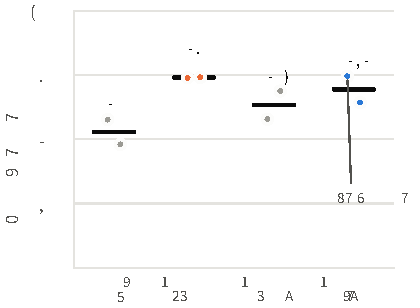
\includegraphics[width=\linewidth]{scarcity-en.pdf}
    \caption{E1: completion time of a low-memory foreground job. Dots are blocks, bars are medians. The run with an actual trim (left blue dot) was the slowest.}
    \label{fig:scarcity}
  \end{minipage}\hfill
  \begin{minipage}[b]{0.49\linewidth}
    \centering
    \small
    \begin{tabular}{@{}lrr@{}}
      \toprule
      Condition & Median (ms) & Trims \\
      \midrule
      Ample RAM (reference) & \numScAmb & 0 \\
      Low memory · absent & \numScAbs & 0 \\
      Low memory · observe & \numScDry & 0 \\
      Low memory · live & \numScLive & 1 \\
      \midrule
      Live $-$ absent & \multicolumn{2}{l}{\numScDiff\ ms (\numScDiffPct\%)} \\
      \bottomrule
    \end{tabular}
    \captionof{table}{E1 summary (two runs per condition). Negative means faster.}
    \label{tab:scarcity}
  \end{minipage}
\end{figure}

In an earlier comparison with $\approx$2.5\,GiB still available, trimming reduced a background app's resident memory by a median of $\approx$1{,}055.6\,MiB, yet system available memory rose by only $\approx$13.3\,MiB, and re-accessing that app took 240.5\,ms instead of 54.5\,ms. Resident-size reduction, available memory and responsiveness are different metrics\citep{mswset,russinovich2004}, and here they visibly diverged. We therefore added the rule ``withhold forced trimming while available physical memory is $\ge$1\,GiB''. In an accelerated-idle-clock regression reproduction, median re-access time went from 238.36\,ms to 56.94\,ms after the fix. This shows that an unnecessary reclaim cost was prevented, not that low-memory performance improved.

\finding{\textbf{Answer to RQ1.} Working-set trimming can raise the available-memory figure, but in these experiments it did not speed up foreground work, and while headroom remained it slowed returning apps. We therefore moved the design's centre from ``emptying memory'' to ``explicit background yielding''.}

\subsection{RQ2: explicit yielding sharply cut p95 under controlled load}
\label{sec:rq2}

\begin{figure}[t]
  \centering
  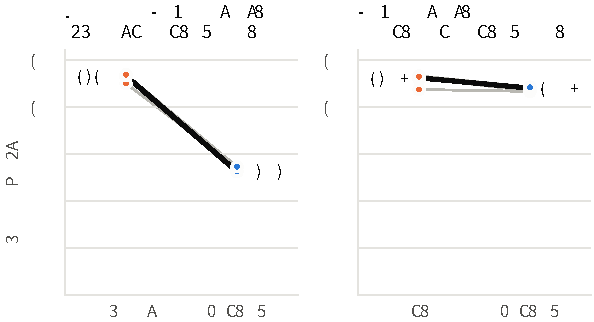
\includegraphics[width=0.66\linewidth]{background-control-en.pdf}
  \caption{E2: per-block foreground request p95. Under memory + CPU contention all five blocks dropped sharply; with CPU contention only (the previous engine made zero adjustments) the difference was small.}
  \label{fig:bgc}
\end{figure}

\begin{table}[t]
\centering\footnotesize
\setlength{\tabcolsep}{3.5pt}
\begin{tabular}{@{}lrrrrrr@{}}
\toprule
& \multicolumn{2}{c}{median p50 (ms)} & \multicolumn{2}{c}{median p95 (ms)} & p95 change & background \\
\cmidrule(lr){2-3}\cmidrule(lr){4-5}
Comparison & base & revised & base & revised & {\scriptsize [block range]} & throughput \\
\midrule
Memory+CPU (absent vs revised) & \numMxOffFifty & \numMxOnFifty & \numMxOff & \numMxOn & $-$\numMxRed\%\ {\scriptsize[\numMxBlkMin, \numMxBlkMax]} & $-$\numMxBgRed\% \\
CPU only (previous vs revised) & \numCpOffFifty & \numCpOnFifty & \numCpOff & \numCpOn & $-$\numCpRed\%\ {\scriptsize[\numCpBlkMin, \numCpBlkMax]} & $-$\numCpBgRed\% \\
\bottomrule
\end{tabular}
\caption{E2 results (five blocks each, 60 requests per condition per block). p95 fell in 5/5 blocks in both comparisons; block ranges are reductions in \%.}
\label{tab:bgc}
\end{table}

In Table~\ref{tab:bgc} and Figure~\ref{fig:bgc}, the median p95 under memory + CPU contention fell from \numMxOff\,ms to \numMxOn\,ms (\numMxRed\%). Per-block reductions clustered tightly at \numMxBlkMin--\numMxBlkMax\%, and the 95\% CI of the geometric-mean reduction was [\numMxGmLo, \numMxGmHi]\%. In every revised condition, all eight background processes were actually adjusted. Available memory just before the task ranged over \numMxAvLo--\numMxAvHi\,MiB.

The CPU-only comparison is instructive. The median (p50) fell from \numCpOffFifty\,ms to \numCpOnFifty\,ms (\numCpFiftyRed\%), but p95 fell by only \numCpRed\%: most requests became faster while the slowest stayed slow. Reporting only means or medians would overstate the effect\citep{dean2013tail}; we report this result rather than omit it. Whether the tail reduction under memory pressure comes from memory priority or from its combination with CPU priority and EcoQoS cannot be separated by this design (\S\ref{sec:threats}).

\finding{\textbf{Answer to RQ2.} Under controlled contention for both memory and CPU, making designated background work yield cut foreground p95 by $\approx$40--44\% in 5/5 blocks. With CPU contention alone the median fell but the tail barely moved.}

\subsection{RQ3: the effect transferred to real Chrome and VS Code}
\label{sec:rq3}

\begin{figure}[t]
  \centering
  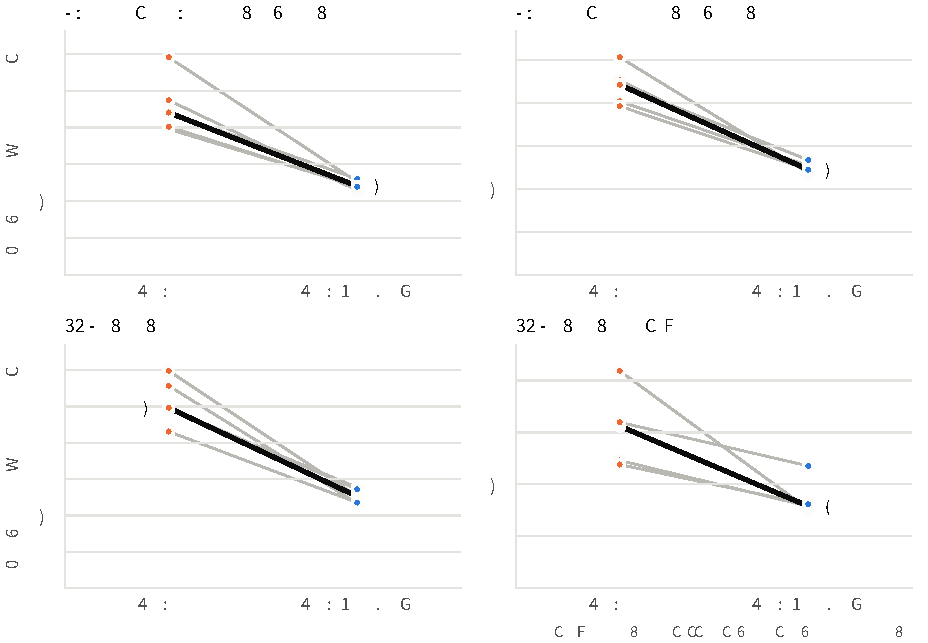
\includegraphics[width=0.92\linewidth]{real-apps-en.pdf}
  \caption{E3: per-block p95 of real application features. All four features improved in all five pairs.}
  \label{fig:real}
\end{figure}

\begin{table}[t]
\centering\footnotesize
\setlength{\tabcolsep}{3pt}
\begin{tabular}{@{}lrrrrrc@{}}
\toprule
& \multicolumn{2}{c}{median p95 (ms)} & & & geo-mean reduction & improved \\
\cmidrule(lr){2-3}
Feature & without & with & reduction & block range & 95\% CI & blocks \\
\midrule
Chrome search $\rightarrow$ render & \numCSOff & \numCSOn & \numCSRed\% & \numCSBlkMin--\numCSBlkMax\% & [\numCSGmLo, \numCSGmHi]\% & 5/5 \\
Chrome sort $\rightarrow$ render & \numCOOff & \numCOOn & \numCORed\% & \numCOBlkMin--\numCOBlkMax\% & [\numCOGmLo, \numCOGmHi]\% & 5/5 \\
VS Code edit $\rightarrow$ completion & \numVCOff & \numVCOn & \numVCRed\% & \numVCBlkMin--\numVCBlkMax\% & [\numVCGmLo, \numVCGmHi]\% & 5/5 \\
VS Code edit $\rightarrow$ save & \numVSOff & \numVSOn & \numVSRed\% & \numVSBlkMin--\numVSBlkMax\% & [\numVSGmLo, \numVSGmHi]\% & 5/5 \\
\bottomrule
\end{tabular}
\caption{E3 results. Each value is the median over five blocks of the per-session p95 of 30 operations. Per-feature exact one-sided sign test $p=\numSignP$.}
\label{tab:real}
\end{table}

In Table~\ref{tab:real} and Figure~\ref{fig:real}, p95 latency of the four features fell by \numCSRed--\numVSRed\%. All five blocks improved, so the per-feature exact one-sided sign test gives $p=\numSignP$; with five blocks the two-sided Wilcoxon test is pinned at its minimum $p=\numWilP$. Because features share sessions, we also pooled by \emph{app session}, the independent unit: in all \numSessions{} sessions every feature improved, two-sided sign test $p=\numPooledP$.

Chrome values include the automation round trip. The in-page p95 from input event to the second rAF boundary moved the same way: search \numEfSOff$\rightarrow$\numEfSOn\,ms, sort \numEfOOff$\rightarrow$\numEfOOn\,ms. Latencies without RamFlow (62--99\,ms) sit near the 0.1\,s limit for a response to feel immediate\citep{card1991}, and with RamFlow (32--51\,ms) clearly below it. The second rAF is a rendering-opportunity boundary, not guaranteed display; VS Code values are API completion times, not keystroke-to-popup times.

\finding{\textbf{Answer to RQ3.} The effect seen under controlled load transferred to a real browser renderer and editor features: p95 fell by $\approx$45--49\% for all four features in 5/5 blocks.}

\subsection{RQ4: the cost is background throughput, and changes were restored safely}
\label{sec:rq4}

\begin{figure}[t]
  \centering
  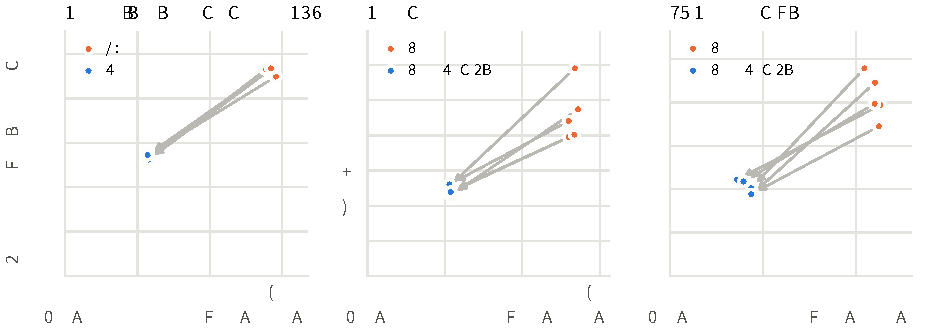
\includegraphics[width=\linewidth]{tradeoff-en.pdf}
  \caption{Foreground responsiveness traded for background throughput. Each arrow moves one block from without (orange) to with (blue). Every point moves down and left: the foreground gets faster and the background slower.}
  \label{fig:tradeoff}
\end{figure}

Figure~\ref{fig:tradeoff} condenses the central result. Background throughput (64\,KiB chunks per second) fell by \numMxBgRed\% in E2, by \numBgCRed\% with Chrome (\numBgCOff$\rightarrow$\numBgCOn) and by \numBgVRed\% with VS Code (\numBgVOff$\rightarrow$\numBgVOn) in E3. RamFlow did not increase total throughput; it changed \emph{who uses resources first}. These are progress rates during the foreground task window and should not be read as proportional increases in background completion time. ProBalance's documentation states that background jobs complete in nearly the same time when deprioritised\citep{probalance}; our load, which contends continuously for CPU and memory, shows that background progress can slow substantially. RamFlow therefore never lifts default protections wholesale and lets the user designate, by executable path, which work \emph{may} yield.

\paragraph{Safety and correctness}
Across the 40 main conditions of E2 and E3 --- 2{,}400 foreground requests and feature operations --- we confirmed: zero out-of-scope change requests; zero safety releases; priority, power and CPU Set values restored to their originals in every condition; identical result hashes for E2's 1{,}200 requests; all E3 search/sort results and completion fields valid; identical final save hashes for each VS Code pair; and unchanged application executable hashes before and after. The measured Core's SHA-256 was \code{d64160b8\ldots8b93} in both E2 and E3, and no policy or binary was changed for these measurements. Automated regression checks passed 218 assertions including Windows API, IPC and real queue child processes, plus 26 storage, 38 external-observer and 70 legacy Python tests.

\finding{\textbf{Answer to RQ4.} The $\approx$45\% foreground p95 reduction cost a $\approx$60\% reduction in designated background throughput. Every adjustment was restored to its original value, with no out-of-scope changes.}

%=====================================================================
\section{Discussion}
\label{sec:discussion}

\paragraph{``Available RAM'' is a metric, not a goal}
E1 and the preceding comparison re-confirm the long-standing critique of RAM optimizers\citep{russinovich2004} on Windows~11. The available-memory figure is easy to raise; what users want is a fast response from the app in use. The quantity to measure is foreground latency, and any action that raises the figure must be measured together with its cost (re-access latency).

\paragraph{Who should wait?}
Under scarcity, the only lever is ordering. Our results show that deferring work the user marked as able to wait cuts foreground tail latency substantially. Guessing this automatically risks harming important background work (recording, downloads, builds), so automatic management stays conservative (30-minute idleness, activity checks) and aggressive yielding is reserved for explicit designation.

\paragraph{Medians and tails move differently}
In the CPU-only comparison p50 fell by 43\% but p95 by 4.8\%. Evaluating responsiveness tools by mean or median alone can exaggerate perceived benefit. We fixed the tail as the primary metric and published unfavourable results as well.

\paragraph{Porting to other systems}
On Linux, PSI provides stall time directly\citep{psi} and cgroup v2 can weight memory and CPU per group of processes, offering a more accurate signal for the same policy\citep{weiner2022tmo}. A Linux edition of RamFlow is being developed in a separate repository and is outside the scope of these measurements.

%=====================================================================
\section{Threats to Validity}
\label{sec:threats}

\paragraph{External validity}
All measurements come from one PC (24\,GiB, hybrid CPU). Results may differ on 8\,GiB machines, other CPUs or laptops on battery. The background load is synthetic SHA-256 work, not real builds, downloads or AI inference. In E3 the foreground apps are real, but they ran generated local pages and documents, not ordinary websites or personal projects.

\paragraph{Construct validity}
The Chrome metric includes the automation round trip and does not guarantee display; the VS Code metric is API completion time. Physical input latency, frame latency and game FPS were not measured. Background throughput is the progress rate during the foreground window.

\paragraph{Internal validity}
The with condition of E2/E3 changed memory priority, CPU priority and EcoQoS together, so their individual contributions cannot be separated. The with condition includes the real engine and tray and their memory cost, but the engine ran in a measurement test host (sensors, policy, setters and restoration were the production code paths). Allocations were not re-matched per condition, so available memory before each task varied with Windows' natural reclaim (recorded in the CSV). E1 had only two blocks with unequal pressure.

\paragraph{Statistical conclusion validity}
Each comparison has five blocks. A 5/5 pattern is strong evidence of consistency, but the minimum two-sided exact $p$ is 0.0625, so no single feature can pass a two-sided 0.05 threshold. The session-level pooled sign test ($p=\numPooledP$) is a conservative grouping that avoids cross-feature correlation. Several features were tested without multiplicity correction. The large, consistent effect sizes make a reversal unlikely, but replication on more PCs and blocks is needed\citep{kalibera2013}.

%=====================================================================
\section{Conclusion}
\label{sec:conclusion}

RamFlow abandons the goal of ``free as much RAM as possible'' in favour of ``protect the task in use and respond to pressure conservatively''. Measurements showed that a trim-centric policy gave no foreground benefit, whereas asking user-designated background work to yield reversibly reduced p95 latency by $\approx$44--49\% under controlled load and in real Chrome and VS Code, at the cost of $\approx$60\% background throughput. Future work: (i) separate the contributions of memory priority, CPU priority and EcoQoS; (ii) policies that tune the degree of yielding continuously; (iii) multi-machine replication including fast app switching and 8\,GiB-class PCs; and (iv) comparison with a PSI-based Linux edition.

{\small
\begin{thebibliography}{99}

\bibitem{denning1968}
P.~J. Denning.
\newblock The working set model for program behavior.
\newblock \emph{Communications of the ACM}, 11(5):323--333, 1968.

\bibitem{mswset}
Microsoft.
\newblock Working set.
\newblock Win32 documentation, \url{https://learn.microsoft.com/en-us/windows/win32/memory/working-set}.

\bibitem{russinovich2004}
M.~Russinovich.
\newblock The memory-optimization hoax: {RAM} optimizers make false promises.
\newblock \emph{Windows IT Pro}, Jan.\ 2004.
\newblock \url{https://www.itprotoday.com/cloud-computing/memory-optimization-hoax}.

\bibitem{chen2021softram}
R.~Chen.
\newblock Analysis of {SoftRAM 95}.
\newblock \emph{The Old New Thing}, Microsoft DevBlogs, Nov.\ 2021.
\newblock \url{https://devblogs.microsoft.com/oldnewthing/20211111-00/?p=105897}.

\bibitem{win10compression}
Microsoft Windows Insider Program.
\newblock Windows 10: Memory compression.
\newblock Windows Insider Hub, Aug.\ 2015 (build 10525).

\bibitem{mavericks2013}
Apple Inc.
\newblock {OS X Mavericks}: Core technologies overview (Compressed Memory, App Nap).
\newblock Technology overview, 2013.

\bibitem{powerthrottling2017}
B.~Karagounis.
\newblock Introducing power throttling.
\newblock Windows Blogs, Apr.\ 2017.
\newblock \url{https://blogs.windows.com/windowsexperience/2017/04/18/introducing-power-throttling/}.

\bibitem{ecoqos2021}
R.~Li.
\newblock Introducing {EcoQoS}.
\newblock Microsoft DevBlogs (Sustainable Software), 2021.
\newblock \url{https://devblogs.microsoft.com/sustainable-software/introducing-ecoqos/}.

\bibitem{mssetprocinfo}
Microsoft.
\newblock {SetProcessInformation} function (processthreadsapi.h).
\newblock Win32 documentation, \url{https://learn.microsoft.com/windows/win32/api/processthreadsapi/nf-processthreadsapi-setprocessinformation}.

\bibitem{mscpusets}
Microsoft.
\newblock {CPU} sets.
\newblock Win32 documentation, \url{https://learn.microsoft.com/windows/win32/procthread/cpu-sets}.

\bibitem{mspriority}
Microsoft.
\newblock {SetPriorityClass} function (processthreadsapi.h).
\newblock Win32 documentation, \url{https://learn.microsoft.com/windows/win32/api/processthreadsapi/nf-processthreadsapi-setpriorityclass}.

\bibitem{mspipe}
Microsoft.
\newblock Named pipe security and access rights.
\newblock Win32 documentation, \url{https://learn.microsoft.com/windows/win32/ipc/named-pipe-security-and-access-rights}.

\bibitem{probalance}
Bitsum.
\newblock {ProBalance} --- Process Lasso documentation.
\newblock \url{https://bitsum.com/apps/process-lasso/docs/algorithms/probalance/}.

\bibitem{weiner2022tmo}
J.~Weiner, N.~Agarwal, D.~Schatzberg, L.~Yang, H.~Wang, B.~Sanouillet, B.~Sharma, T.~Heo, M.~Jain, C.~Tang, and D.~Skarlatos.
\newblock {TMO}: Transparent memory offloading in datacenters.
\newblock In \emph{Proc.\ ASPLOS '22}, 2022.
\newblock \url{https://doi.org/10.1145/3503222.3507731}.

\bibitem{psi}
The Linux kernel documentation.
\newblock {PSI} --- Pressure stall information.
\newblock \url{https://docs.kernel.org/accounting/psi.html}.

\bibitem{lmkd}
Android Open Source Project.
\newblock Low memory killer daemon.
\newblock \url{https://source.android.com/docs/core/perf/lmkd}.

\bibitem{dean2013tail}
J.~Dean and L.~A. Barroso.
\newblock The tail at scale.
\newblock \emph{Communications of the ACM}, 56(2):74--80, 2013.

\bibitem{card1991}
S.~K. Card, G.~G. Robertson, and J.~D. Mackinlay.
\newblock The information visualizer, an information workspace.
\newblock In \emph{Proc.\ CHI '91}, pages 181--186, 1991.

\bibitem{mytkowicz2009}
T.~Mytkowicz, A.~Diwan, M.~Hauswirth, and P.~F. Sweeney.
\newblock Producing wrong data without doing anything obviously wrong!
\newblock In \emph{Proc.\ ASPLOS XIV}, pages 265--276, 2009.

\bibitem{kalibera2013}
T.~Kalibera and R.~Jones.
\newblock Rigorous benchmarking in reasonable time.
\newblock In \emph{Proc.\ ISMM '13}, pages 63--74, 2013.

\bibitem{jain1991}
R.~Jain.
\newblock \emph{The Art of Computer Systems Performance Analysis}.
\newblock Wiley, 1991.

\bibitem{cdp}
Chrome for Developers.
\newblock Changes to remote debugging switches to improve security.
\newblock \url{https://developer.chrome.com/blog/remote-debugging-port}.

\bibitem{vscodetest}
Visual Studio Code.
\newblock Testing extensions; Built-in commands.
\newblock \url{https://code.visualstudio.com/api/working-with-extensions/testing-extension}.

\end{thebibliography}

}

\appendix
\section{Reproduction}
\label{app:repro}
Per-condition summary CSVs and protocol/hash JSON live under \code{docs/evidence/}. Every number (\code{paper/shared/numbers.tex}) and figure (\code{paper/figures/}) in this report is regenerated by:
\begin{center}
\small\code{python3 paper/analysis/analyze.py}\qquad\code{cd paper/en \&\& xelatex main \&\& xelatex main}
\end{center}
Analysis needs Python~3, numpy, scipy and matplotlib; typesetting needs XeLaTeX and the Noto CJK fonts. Raw measurement records (per-request logs, raw sensors, events, run sources) are excluded from Git for size and kept locally under \code{benchmarks/}; the summary CSVs are the input to the analysis here. Product build and regression instructions are in the repository \code{README.md}.

\begin{table}[h]
\centering\small
\begin{tabularx}{\linewidth}{@{}lX@{}}
\toprule
Data & Location \\
\midrule
E1 low memory & \code{docs/evidence/2026-11-09-scarcity/\{trials.csv, summary.json\}} \\
E2 background control & \code{docs/evidence/2026-11-09-background-control/\{trials.csv, summary.json\}} \\
E3 real apps & \code{docs/evidence/2026-11-10-real-apps/\{trials.csv, summary.json\}} \\
Derived statistics & \code{paper/analysis/stats.json} \\
Policy code & \code{native/RamFlow.Core/Policy.cs}, \code{Engine.cs}, \code{BackgroundJobs.cs} \\
\bottomrule
\end{tabularx}
\end{table}

\end{document}
